%        File: paper.tex
%     Created: Fri Jun 23 06:00 PM 2017 J
% Last Change: Fri Jun 23 06:00 PM 2017 J
%
%%% jdummy.def
%
\DeclareRelationFont{JY1}{mc}{it}{}{OT1}{cmr}{it}{}
\DeclareRelationFont{JT1}{mc}{it}{}{OT1}{cmr}{it}{}
\DeclareFontShape{JY1}{mc}{m}{it}{<5> <6> <7> <8> <9> <10> sgen*min
    <10.95><12><14.4><17.28><20.74><24.88> min10
    <-> min10}{}
\DeclareFontShape{JT1}{mc}{m}{it}{<5> <6> <7> <8> <9> <10> sgen*tmin
    <10.95><12><14.4><17.28><20.74><24.88> tmin10
    <-> tmin10}{}
\DeclareRelationFont{JY1}{mc}{sl}{}{OT1}{cmr}{sl}{}
\DeclareRelationFont{JT1}{mc}{sl}{}{OT1}{cmr}{sl}{}
\DeclareFontShape{JY1}{mc}{m}{sl}{<5> <6> <7> <8> <9> <10> sgen*min
    <10.95><12><14.4><17.28><20.74><24.88> min10
    <-> min10}{}
\DeclareFontShape{JT1}{mc}{m}{sl}{<5> <6> <7> <8> <9> <10> sgen*tmin
    <10.95><12><14.4><17.28><20.74><24.88> tmin10
    <-> tmin10}{}
\DeclareRelationFont{JY1}{mc}{sc}{}{OT1}{cmr}{sc}{}
\DeclareRelationFont{JT1}{mc}{sc}{}{OT1}{cmr}{sc}{}
\DeclareFontShape{JY1}{mc}{m}{sc}{<5> <6> <7> <8> <9> <10> sgen*min
    <10.95><12><14.4><17.28><20.74><24.88> min10
    <-> min10}{}
\DeclareFontShape{JT1}{mc}{m}{sc}{<5> <6> <7> <8> <9> <10> sgen*tmin
    <10.95><12><14.4><17.28><20.74><24.88> tmin10
    <-> tmin10}{}
\DeclareRelationFont{JY1}{gt}{it}{}{OT1}{cmbx}{it}{}
\DeclareRelationFont{JT1}{gt}{it}{}{OT1}{cmbx}{it}{}
\DeclareFontShape{JY1}{mc}{bx}{it}{<5> <6> <7> <8> <9> <10> sgen*goth
    <10.95><12><14.4><17.28><20.74><24.88> goth10
    <-> goth10}{}
\DeclareFontShape{JT1}{mc}{bx}{it}{<5> <6> <7> <8> <9> <10> sgen*tgoth
    <10.95><12><14.4><17.28><20.74><24.88> tgoth10
    <-> tgoth10}{}
\DeclareRelationFont{JY1}{gt}{sl}{}{OT1}{cmbx}{sl}{}
\DeclareRelationFont{JT1}{gt}{sl}{}{OT1}{cmbx}{sl}{}
\DeclareFontShape{JY1}{mc}{bx}{sl}{<5> <6> <7> <8> <9> <10> sgen*goth
    <10.95><12><14.4><17.28><20.74><24.88> goth10
    <-> goth10}{}
\DeclareFontShape{JT1}{mc}{bx}{sl}{<5> <6> <7> <8> <9> <10> sgen*tgoth
    <10.95><12><14.4><17.28><20.74><24.88> tgoth10
    <-> tgoth10}{}
\DeclareRelationFont{JY1}{gt}{sc}{}{OT1}{cmbx}{sc}{}
\DeclareRelationFont{JT1}{gt}{sc}{}{OT1}{cmbx}{sc}{}
\DeclareFontShape{JY1}{mc}{bx}{sc}{<5> <6> <7> <8> <9> <10> sgen*goth
    <10.95><12><14.4><17.28><20.74><24.88> goth10
    <-> goth10}{}
\DeclareFontShape{JT1}{mc}{bx}{sc}{<5> <6> <7> <8> <9> <10> sgen*tgoth
    <10.95><12><14.4><17.28><20.74><24.88> tgoth10
    <-> tgoth10}{}
\DeclareRelationFont{JY1}{gt}{it}{}{OT1}{cmr}{it}{}
\DeclareRelationFont{JT1}{gt}{it}{}{OT1}{cmr}{it}{}
\DeclareFontShape{JY1}{gt}{m}{it}{<5> <6> <7> <8> <9> <10> sgen*goth
    <10.95><12><14.4><17.28><20.74><24.88> goth10
    <-> goth10}{}
\DeclareFontShape{JT1}{gt}{m}{it}{<5> <6> <7> <8> <9> <10> sgen*tgoth
    <10.95><12><14.4><17.28><20.74><24.88> tgoth10
    <-> tgoth10}{}
\endinput
%%%% end of jdummy.def

\documentclass[submit,techrep]{ipsj_v2/UTF8/ipsj}

\usepackage{latexsym}
\usepackage[dvipdfmx]{graphicx}
\usepackage{amssymb}
\usepackage{enumerate,cite,url}
\usepackage{listings,jlisting}
\lstset{%
    language={c},%
    basicstyle={\small\ttfamily},%
    identifierstyle={\small},%
    commentstyle={\scriptsize\itshape},%
    keywordstyle={\small},%\bfseries},%
    ndkeywordstyle={\small},%
    stringstyle={\small\it},
    frame={tb},
    breaklines=true,
    columns=[l]{fullflexible},%
    numbers=left,%
    xrightmargin=0zw,%
    xleftmargin=3zw,%
    numberstyle={\scriptsize},%
    stepnumber=1,
    numbersep=1zw,%
    lineskip=-0.5ex%
}

\begin{document}

\title{
    {\Huge 組込みシステムに適した動的メモリアロケータのコンポーネント化}
  \\{\huge Componentized Dynamic Memory Allocator for Embedded Systems}
}

\etitle{\vspace{-3.5cm}}
% \etitle{Componentized Dynamic Memory Allocator for Embedded Systems}

\affiliate{OU}{大阪大学基礎工学研究科\\
Graduate School of Engineering Science, Osaka University}

\affiliate{OKUMA}{オークマ株式会社\\
OKUMA Corporation}

\author{ {\LARGE 山本 拓朗}}{{\Large Takuro Yamamoto}}{OU}%[joho.taro@ipsj.or.jp]
\author{  {\LARGE 大山 博司}}{{\Large Hiroshi Oyama}}{OKUMA}%
\author{  {\LARGE 安積 卓也}}{{\Large Takuya Azumi}}{OU}%[gakkai.jiro@ipsj.or.jp]

\maketitle

\section{はじめに}

近年,組込みシステムは多くの機器に組み込まれており,このIoT社会を支える重要な役割を担っている\cite{par:IoTIndustries}\cite{par:IoTComputing}.
多くの組込みシステムは,厳しいリソース制約を持っており,効率的なメモリ確保が要求される.
さらに,リアルタイム性を要求される組込みシステムでは,メモリ確保の実行時間も重要となる.

このような要求を満たす,組込みシステムに適した動的メモリアロケータとして,TLSF (Two-Level Segregate Fit) アロケータが提案されている\cite{par:TLSF}\cite{url:TLSF}.
TLSFアロケータは,メモリブロックを2段階で分類することでメモリ利用効率を向上させており,常に$O(1)$で実行するため最悪実行時間を見積もることができ,リアルタイムシステムに適した動的メモリアロケータである.
TLSFアロケータは,メモリ利用効率が良く,リアルタイムシステムに向いているため,多くのリアルタイムOSで採用されている.

しかし,現状では,複数のスレッドが並行動作すると,メモリの衝突が起きる場合がある.
本研究では,組込み向けコンポーネントシステムであるTECS (TOPPERS Embedded Component System)\cite{url:TECS}\cite{par:TECS} を用いてTLSFアロケータをコンポーネント化する.
TECSを用いたコンポーネントベース開発は,ソフトウェアの再利用性を向上させ,システムを可視化できるため,ソフトウェア開発の生産性を向上させることができる.
コンポーネント化されたTLSFアロケータは,各コンポーネントが独自のヒープ領域を保持するため,スレッドセーフなメモリアロケータを実現できる.
さらに,コンポーネントとして特性を利用できるため,メモリサイズの変更等が柔軟になる.
本論文では,TLSFメモリアロケータコンポーネントを提案し,そのユースケースとして,利用例を述べる.

本論文における貢献は以下の通りである.
\begin{itemize}
    \item 複数のスレッドが並行動作しても排他制御なしでスレッドセーフに動作する
    \item 各スレッドで独自のヒープ領域を容易に設定できる
    \item コンポーネント化により再利用性が向上するため,様々なシステムに拡張できる
    \item コンポーネント図により可視化できるため,機能役割の理解が容易になる
\end{itemize}

本論文の構成は次の通りである.
まず\ref{sec:ComponentBasedDevelopment}章で,コンポーネントベース開発と提案するアロケータのベースとして用いるTECSについて述べる.
\ref{sec:DesignImplementation}章では,TLSFメモリアロケータのコンポーネント設計と実装について述べる.
\ref{sec:UseCase}章では,ユースケースとして,利用例を述べ, 最後に\ref{sec:Conclusion}章で本論文をまとめる.

\section{コンポーネントベース開発}
\label{sec:ComponentBasedDevelopment}

ソフトウェア開発の生産性を向上させる手法のひとつにコンポーネントベース開発がある\cite{par:Crnkovic}\cite{par:CBD}.
コンポーネントベース開発は,ソフトウェアの部品(コンポーネント)を組み合わせて開発を行う手法である.
ソフトウェアの再利用性が改善する上に,コンポーネント図によりシステム全体の構造を可視化するため,ソフトウェア開発の生産性を向上できる.
さらに,システムの拡張や仕様変更にも柔軟に対応することができる.
組込みシステム向けのコンポーネント技術として,TECSやAUTOSAR\cite{url:AUTOSAR},SaveCCM\cite{par:SaveCCM}がある.
本研究で利用したTECSについて次で述べる.

\subsection{TECS}

TECS (TOPPERS Embedded Component System)は,TOPPERSプロジェクト\cite{url:TOPPERS}で開発されている組込みシステム向けのコンポーネント技術である.
TECSでは,コンポーネントの生成と結合はすべて静的に行われ,最適化されるため,コンポーネント化における実行時間や消費メモリのオーバヘッドを抑えることができる.
さらに,組込みシステム開発に広く用いられているC言語による開発を採用しており,組込みシステムに特化したコンポーネントシステムである.

\subsubsection{コンポーネントモデル}

図\ref{fig:component}にTECSコンポーネント図の例を示す.
TECSでは,インスタンス化されたコンポーネントはセル({\it cell})と呼ばれ,受け口({\it entry}),呼び口({\it call}),属性,変数を持つ.
受け口は自身の機能を提供するインタフェースで,呼び口は他のセルの機能を利用するためのインタフェースである.
セルは複数の受け口や呼び口を持つことができる.
セルの提供する関数は,C言語で実装される.

受け口と呼び口の型は,セルの機能を使うためのインタフェースであるシグニチャによって定義される.
セルの呼び口は,同じシグニチャを持つ他のセルの受け口と結合できる.
セルの型は,セルタイプと呼ばれ,受け口,呼び口,属性,変数の組を定義している.

\begin{figure}[t]
    \centering
    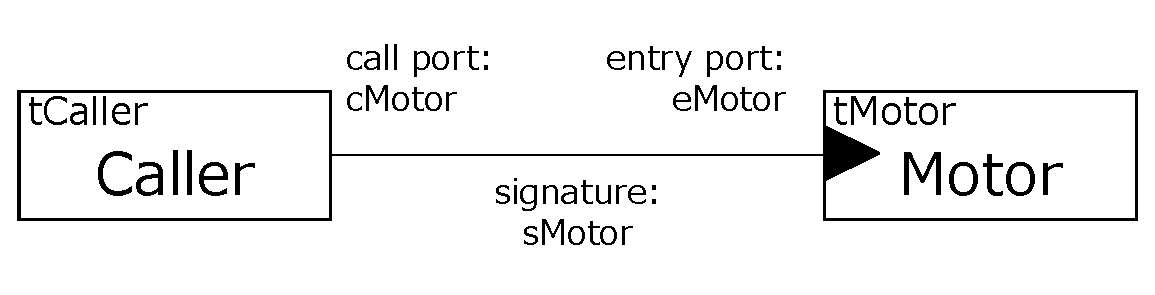
\includegraphics[width=8cm,clip]{figure/component_diagram.pdf}
    \caption{TECSコンポーネント図の例}
    \label{fig:component}
\end{figure}

\subsubsection{コンポーネント記述}
TECSのコンポーネント記述は,シグニチャ記述,セルタイプ記述,組上げ記述に分類され,CDL (Component Description Language)ファイルに記述する.
図\ref{fig:component}のコンポーネント記述について次に述べる.

\begin{description}
    \item[{\bf シグニチャ記述}]\mbox{}\\
        シグニチャ記述は,セルのインタフェースを定義する.
        図\ref{signature}に示す通り,{\it signature}キーワードに続けて,シグニチャ名(sMotor)を記述する.
        %図\ref{signature}のようにシグニチャsMotorを定義できる.
        TECSでは,インタフェースの定義を明確にするために,入力と出力にはそれぞれ,[in]と[out]という指定子が付けられる.
        
\begin{figure}[t]
\centering
\begin{lstlisting}
signature sMotor {
    void initializePort( [in]int32_t type );
    int32_t getCounts( void );
    ER resetCounts( void );
    ER setPower( [in]int power );
    ER stop( [in] bool_t brake );
    ER rotate( [in] int degrees,
                [in] uint32_t speed_abs,
                [in] bool_t blocking );
};
\end{lstlisting}
\caption{シグニチャ記述}
\label{signature}
\end{figure}

    \item[{\bf セルタイプ記述}]\mbox{}\\
        セルタイプ記述は,受け口,呼び口,属性,変数を用いてセルタイプを定義する.
        {\it celltype}キーワードに続けて,セルタイプ名(tCaller)を記述する.
        図\ref{celltype}に示す通り,受け口は,{\it entry}キーワードに続けて,シグニチャ名,受け口名を記述する.
        同様にして,呼び口も定義できる.
        属性と変数は,それぞれ{\it attr},{\it var}キーワードを用いて列挙する.

\begin{figure}[t]
\centering
\begin{lstlisting}
celltype tCaller {
    call sMotor cMotor;
};
celltype tMotor {
    entry sMotor eMotor;
    attr {
        int32_t port;
    };
    var {
        int32_t currentSpeed = 0;
    };
};
\end{lstlisting}
\caption{セルタイプ記述}  
\label{celltype}
\end{figure}

    \item[{\bf 組上げ記述}]\mbox{}\\
        組上げ記述は,セルをインスタンス化し,セルを結合する.
        {\it cell}キーワードに続けて,セルタイプ名,セル名を記述する.
        呼び口名,``=",結合先の受け口名の順に記述し,セルを結合する.
        図\ref{build}では,セルCallerの呼び口cMotorと,セルMotorの受け口eMotorが結合されている.
        
\begin{figure}[t]
\centering
\begin{lstlisting}
cell tMotor Motor {
};
cell tCaller Caller {
    cMotor = Motor.eMotor;
};
\end{lstlisting}
\caption{組上げ記述}
\label{build}
\end{figure}

\end{description}

\subsubsection{開発フロー}

図\ref{fig:DevelopmentFlow}にTECSを利用した開発フローを示す.
TECSジェネレータは,CDLファイルから,C言語のインターフェースコード(.hや.c)とリアルタイムOSのシステム設定ファイル(.cfg)を生成する.

TECSを用いたソフトウェア開発者は,コンポーネント設計者とアプリケーション開発者に分けられる.
コンポーネント設計者は,セル間のインターフェースであるシグニチャやセルの型であるセルタイプを定義する.
これらが定義されたCDLファイルから生成されたテンプレートコードを利用し,コンポーネントの提供する機能や振る舞いをC言語で実装する.
コンポーネントの機能を実装したソースコードは,セルタイプコードと呼ばれる.
アプリケーション開発者は,コンポーネント図や定義済みのセルタイプを利用して,組上げ記述によりセル同士を結合させることでアプリケーションを開発する.
最終的にヘッダ,インターフェースコード,セルタイプコードをコンパイル・リンクすることで,アプリケーションモジュールが生成される.



\section{設計と実装}
\label{sec:DesignImplementation}


\subsection{TLSF}
\label{sec:TLSF}
TLSF (Two-Level Segregate Fit)メモリアロケータは,M. Masmanoらによって提案されたリアルタイムシステムに適した動的メモリアロケータである.
TLSFメモリアロケータは以下のような特徴がある.
\begin{description}
    \item[{\bf リアルタイム性}]\mbox{}\\
        メモリの確保や解放にかかる最悪実行時間はデータサイズに依存しないため,常に$O(1)$で実行される.
        応答時間を見積もることができるため,リアルタイムシステムに適したメモリアロケータである.
    \item[{高速}]\mbox{}\\
        最悪実行時間が常に見積もれることに加え,TLSFは高速に実行される.
        x86アーキテクチャで最大168のプロセッサ命令を実行することができる.
    \item[{効率的なメモリ消費}]\mbox{}\\
        TLSFでは,メモリの断片化(フラグメンテーション)を抑えることで,メモリ効率化を実現している.
        様々なテストで,平均フラグメンテーション15%未満,最大フラグメンテーション25%未満を得ている.
\end{description}


\subsubsection{TLSFアルゴリズム}

TLSFアルゴリズムは,メモリブロックを2段階に分類して,要求されたメモリサイズに最適なメモリブロックを検索する.
図\ref{fig:TLSF}にTLSFアルゴリズムの概要を示す.
例として,$malloc(100)$というメモリ確保の要求がされた場合を考える.
まず第一段階では,要求されたメモリサイズの最上位ビットで分類する.
この場合,100を2進数で表すと1100100であるため,最上位ビットから64から128の範囲であることが分かる.
次に第二段階では,さらに細かい分類を行う.
今回の場合,64から128を4分割しており,100は96-111のブロックに入る.
この範囲にあるフリーブロック\footnote{フリーブロックは使用可能なメモリブロックのことである.}を使用するという流れである.

単純な固定サイズブロック確保では最大50\%の無駄を生じてしまうが,TLSFでは2段階で細かく分類するため,メモリ効率が良いアルゴリズムとなっている.
また,検索にかかる時間も高速で常に同じ速度で実行される.


\begin{figure}[t]
    \centering
    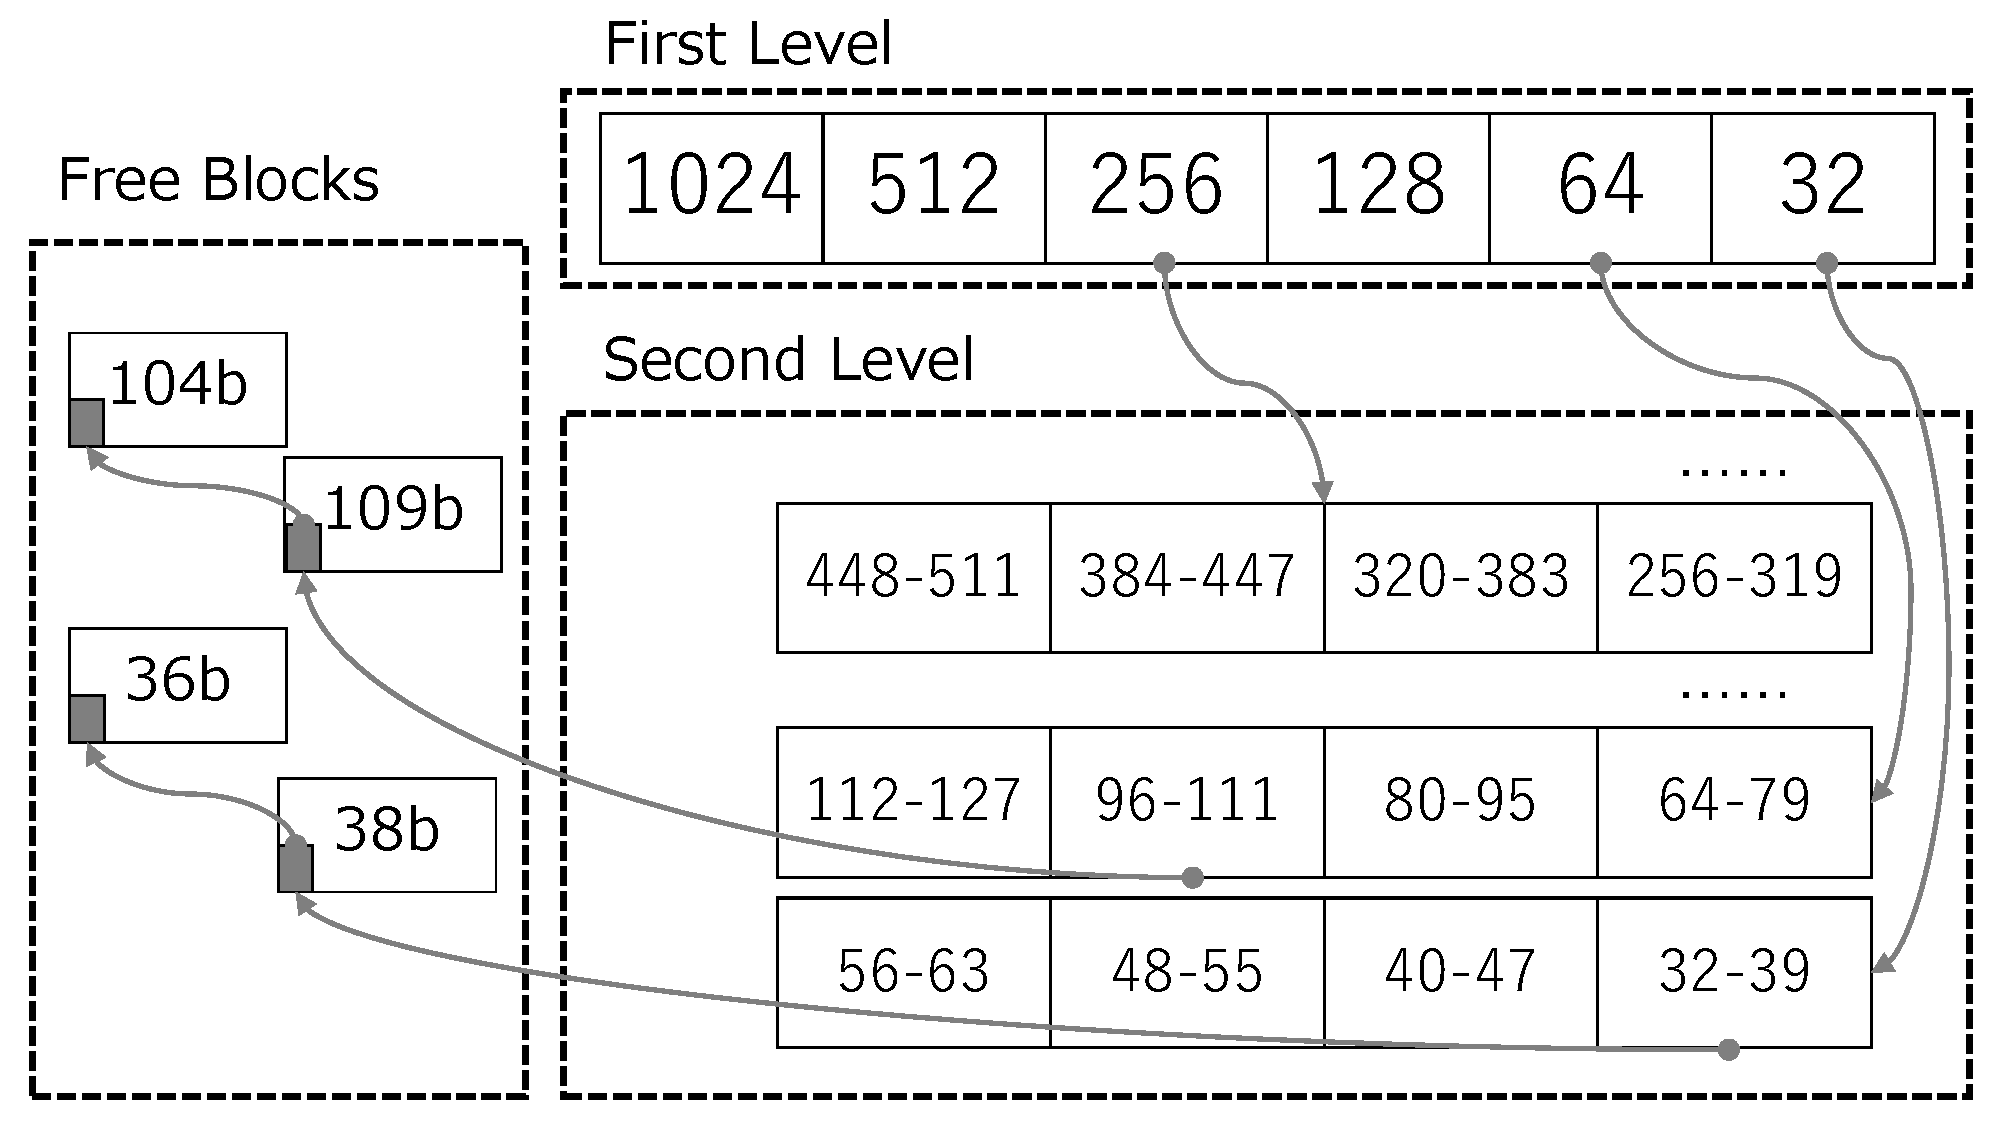
\includegraphics[width=8cm,clip]{figure/TLSF.pdf}
    \caption{TLSFアルゴリズム}
    \label{fig:TLSF}
\end{figure}


\subsection{コンポーネント設計}

TLSFメモリアロケータのコンポーネント設計について述べる.
本研究では,TECSを用いてTLSFをコンポーネント化を行っている.
使用したTLSFのバージョンは,2.4.6である\footnote{http://www.gii.upv.es/tlsf/main/repo}.

\begin{figure}[t]
\centering
\begin{lstlisting}
[deviate]
signature sMalloc {
    int    initializeMemoryPool(void);
    void   *calloc( [in]size_t nelem,
                    [in]size_t elem_size );
    void   *malloc( [in]size_t size );
    void   *realloc( [in]const void *ptr,
                     [in]size_t new_size );
    void   free( [in]const void *ptr );
};
\end{lstlisting}
\caption{メモリ管理用のシグニチャ記述}  
\label{src:TLSFSignature}
\end{figure}


図\ref{src:TLSFSignature}は,アロケータが使用するメモリ管理用のシグニチャ記述である.
メモリプール初期化関数{\it initializeMemoryPool},メモリ確保用の関数{\it calloc}, {\it malloc}, {\it realloc},そしてメモリ解放用の関数{\it free}をシグニチャとして定義している.

\begin{figure}[t]
\centering
\begin{lstlisting}
celltype tTLSFMalloc {
    [inline]
        entry  sMalloc  eMalloc;
    attr {
        /* memory pool size in bytes */
        size_t  memoryPoolSize;
    };
    var {
        [size_is( memoryPoolSize / 8 )]
            uint64_t   *pool;
    };
};
\end{lstlisting}
\caption{TLSFメモリアロケータのセルタイプ記述}  
\label{src:TLSFCelltype}
\end{figure}


TLSFメモリアロケータコンポーネントのセルタイプ記述を図\ref{src:TLSFCelltype}に示す.
受け口{\it eMalloc}は,メモリ管理(確保や解放)を行うすべてのコンポーネントと結合される.
ここで,{\it [inline]}は受け口関数をインライン関数として提供するための指定子である.
メモリプールサイズをコンポーネントの属性として,メモリプールへのポインタをコンポーネントの内部変数として定義している.
各コンポーネントが独自のヒープ領域を保持しているため,異なるスレッドで同時にメモリ管理用の関数を呼び出した場合でも,排他制御を行うことなく,メモリ競合を起こさない.

\begin{figure}[t]
    \centering
    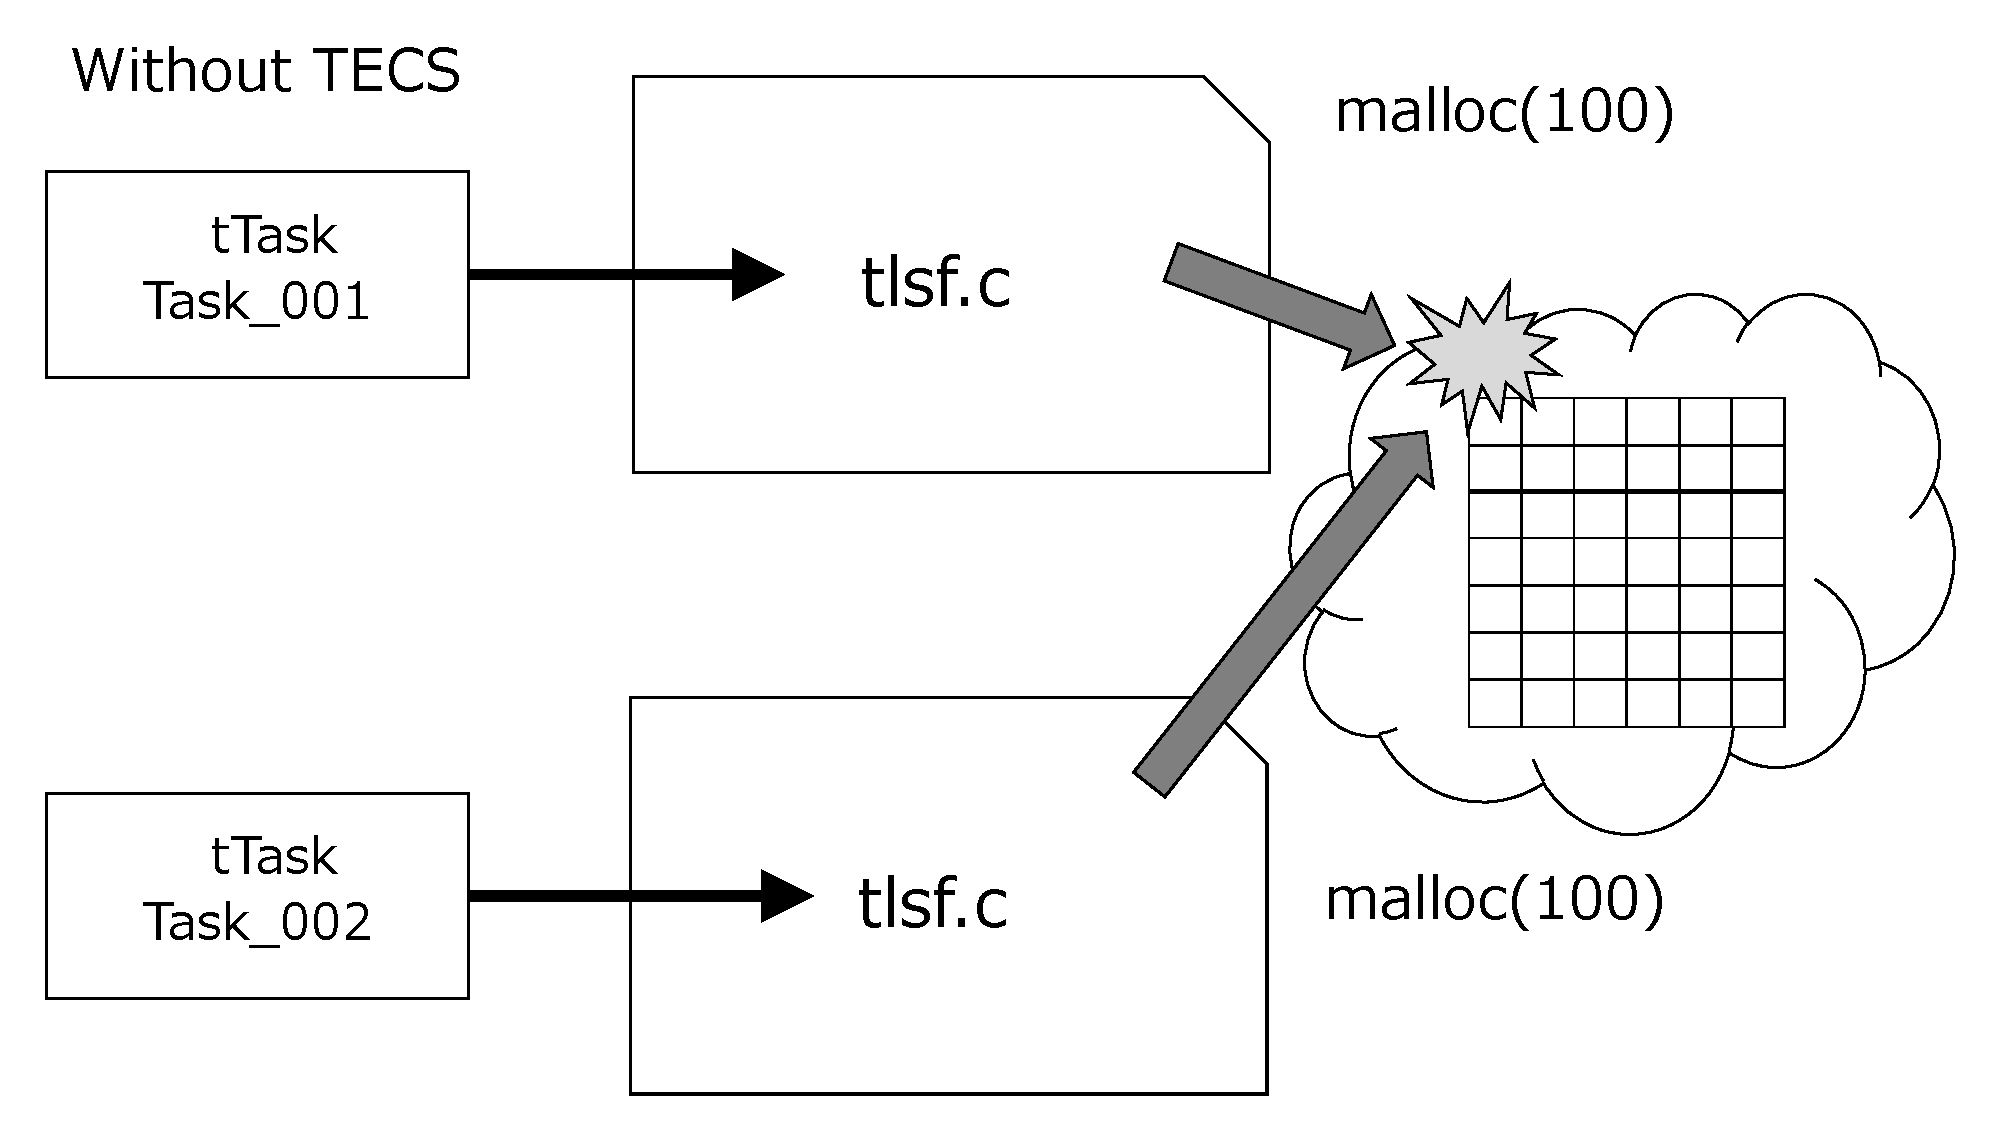
\includegraphics[width=8cm,clip]{figure/WithoutTECS.pdf}
    \caption{コンポーネント化される前のTLSF}
    \label{fig:WithoutTECS}
\end{figure}

\begin{figure}[t]
    \centering
    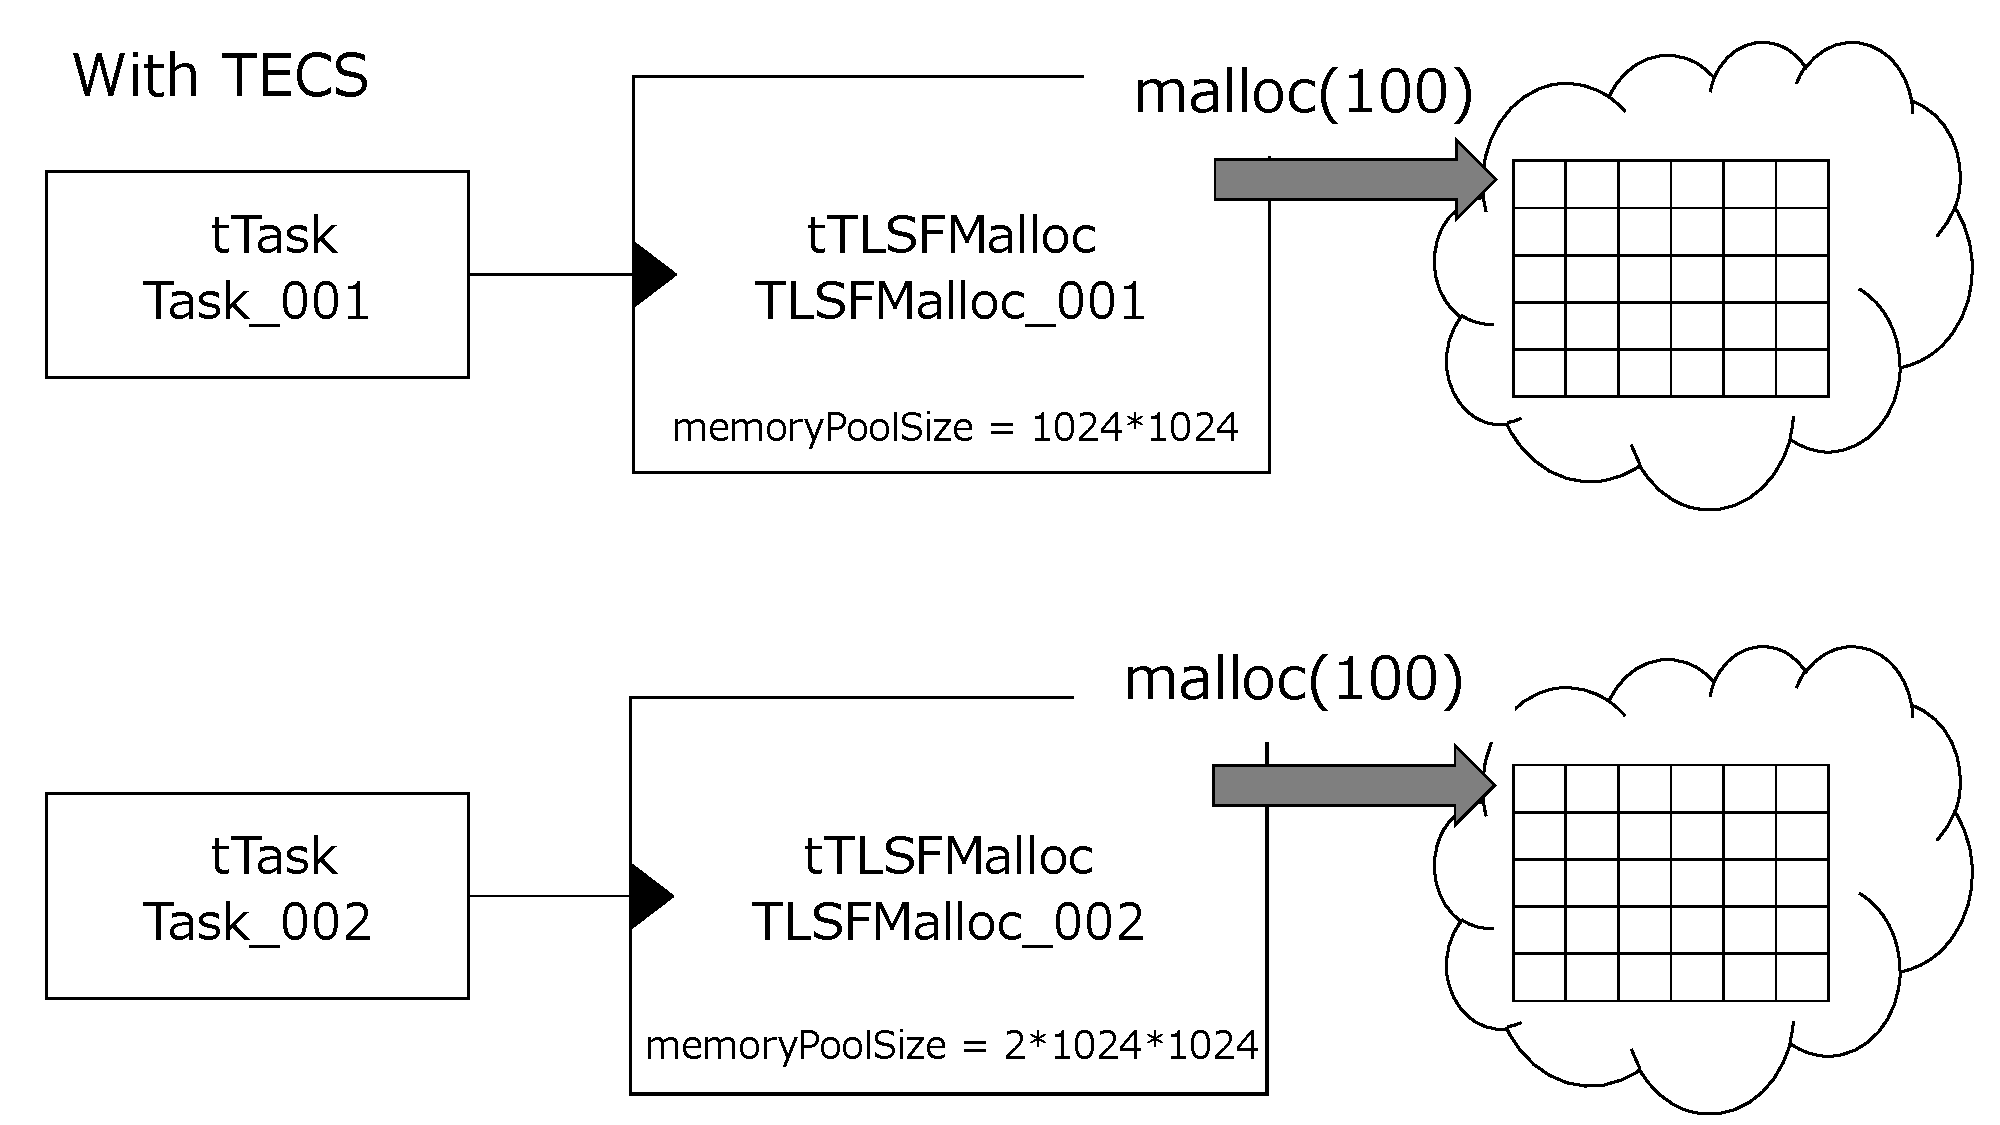
\includegraphics[width=8cm,clip]{figure/WithTECS.pdf}
    \caption{コンポーネント化されたTLSF}
    \label{fig:WithTECS}
\end{figure}

図\ref{fig:WithoutTECS}に示すように,コンポーネント化を行う前のTLSFでは,ヒープ領域を複数のスレッドで共有しているため,複数のスレッドからメモリの確保や解放を同時に行うとメモリ競合が生じる場合があった.
図\ref{fig:WithTECS}のように,TECSを用いてTLSFのコンポーネント化を行うと,各コンポーネントが独自にヒープ領域を保持し,その中でメモリ管理を行うため,排他制御なしでスレッドセーフに動作することが可能になる.

\begin{figure}[t]
\centering
\begin{lstlisting}
void*
mrb_TECS_allocf(mrb_state *mrb, void *p, size_t size, void *ud)
{
    CELLCB	*p_cellcb= (CELLCB *)ud;
    if (size == 0) {
        cMalloc_free(p);
        //tlsf_free(p);
        return NULL;
    }
    else if (p){
        //return tlsf_realloc(p,size);
        return cMalloc_realloc(p, size);
    }
    else {
        //return tlsf_malloc(size);
        return cMalloc_malloc(size);
    }
}
\end{lstlisting}
\caption{TLSFメモリアロケータコンポーネントの利用部分}  
\label{src:TLSFC}
\end{figure}


\section{ユースケース}
\label{sec:UseCase}

本章では,提案するコンポーネント化されたTLSFメモリアロケータのユースケースとして,利用されるプラットフォームとその効果について述べる.

\subsection{mruby on TECS}
\label{sec:mrubyonTECS}

mruby on TECS は,mruby (軽量Ruby)\cite{par:mruby}\cite{url:mruby}を用いたコンポーネントベース開発が可能な組込みソフトウェア開発フレームワークである\cite{par:mrubyonTECS}.
スクリプト言語を用いることで,組込みソフトウェア開発の生産性向上を目指している.
一般に,スクリプト言語は実行速度が遅いため,組込みソフトウェアに向いていないが,mruby on TECSでは,mruby-TECSブリッジの機能によって,mruby プログラムからC 言語の関数を呼び出すことができるため,C言語と変わらない速度でプログラムを実行することができる.
mrubyプログラムは,mrubyコンパイラによってバイトコードに変換され,RiteVMと呼ばれるVM上で実行される.
本フレームワークでは,RiteVMやRTOS (Real-Time OS)の機能もすべてTECSによってコンポーネント化されている.

% 本研究では,RTOS として,TOPPERS/HRP2 [6] を使用した.
% TOPPERS/HRP2 は,$\mu$ITRONをベースにしたメモリ保護機能を持つRTOSである.
% しかし,TECSはTOPPERS/HRP2 だけでなく,OSEKやTOPPERS/ASPといったRTOS にも対応しているため,mruby on TECS はRTOS に依存しない.

\subsubsection{マルチVM対応}

本フレームワークでは,VMが行うメモリ管理にTLSFメモリアロケータを採用している.
しかし,既存のTLSFメモリアロケータではスレッドセーフではないため,複数のスレッドからメモリの確保や解放を行うと,メモリ衝突が起きてしまう.
VMは高い頻度でメモリの確保と解放を繰り返すため,マルチVMとして複数のVMを起動すると,すぐに衝突を起こしてしまう.

図\ref{fig:UseCase_mruby}のように,VMにTLSFメモリアロケータコンポーネントを結合し,各VMで独自のヒープ領域を持つように設計する.
各VMが結合しているTLSFコンポーネントがそれぞれメモリプールを保持しているため,複数のVMがメモリ衝突を起こすことなく,実行できる.
図\ref{fig:UseCase_mruby}では,1つ目のVMが1MB (1024*1024)のヒープ領域,2つ目のVMが2MB (2*1024*1024)のヒープ領域を持っていることを示している.
コンポーネント化により,各VMで異なるヒープ領域を設定することが容易になっている.
さらに,RiteVMはインクリメンタルGC (Garbage Collection)を行うが,独自のメモリプールを保持しているため,GCを始めたVMがGCの実行によって,他のVMの実行を妨げることもない.

\begin{figure}[t]
    \centering
    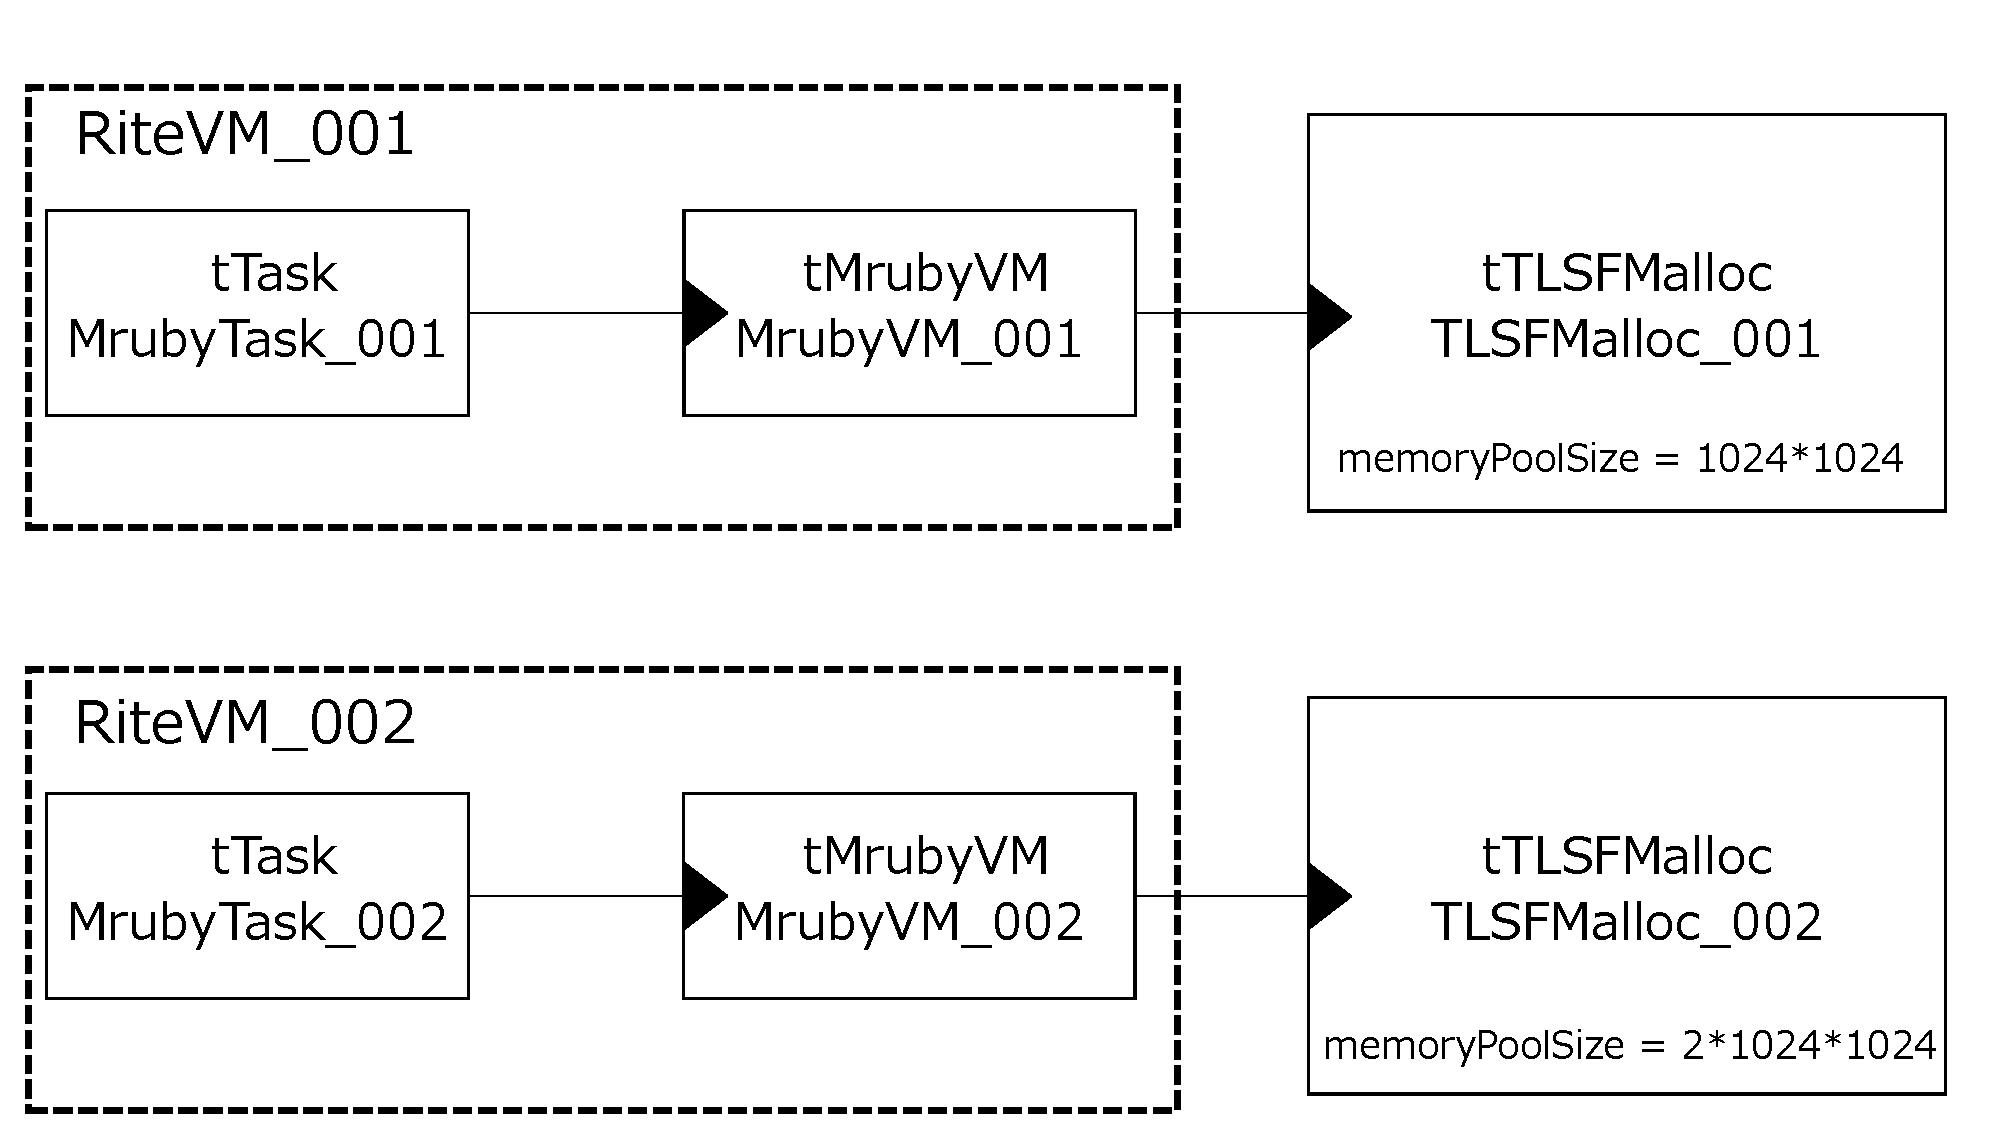
\includegraphics[width=8cm,clip]{figure/UseCase_mruby.pdf}
    \caption{RiteVMとTLSFのコンポーネント図}
    \label{fig:UseCase_mruby}
\end{figure}
    
\subsection{TINET+TECS}
\label{sec:TINET+TECS}

TINET+TECSは,組込み向けのTCP/IPプロトコルスタックであるTINET (Tomakomai InterNETworking)\cite{url:TINET}\cite{par:TINET}をTECSによってコンポーネント化したTCP/IPプロトコルスタックである\cite{par:TINET+TECS}.
複雑で大規模なソースコードやマクロで構成されているTINETをTECSによってコンポーネント化することで,実行時間やメモリ消費量のオーバヘッドを抑えつつ,TCP/UDPやIPv4/IPv6といった通信プロトコルの変更等のコンフィグラビリティが向上している.

\subsubsection{データ送受信用のメモリ管理}

データの送受信処理を行う際,各プロトコルでメモリ領域の確保と解放が行われる.
TINET+TECSやTINETは,プロトコル間のデータコピー回数を最少とするなど,組込みシステムの厳しいメモリ制約に対応している.
しかし,現状ではTOPPERS/ASP\footnote{TOPPERS/ASPは,TOPPERSプロジェクトで開発されている$\mu$ITRON\cite{par:microITRON}をベースにしたリアルタイムOSである.}でサポートされている固定長メモリアロケータを利用している.
TLSFメモリアロケータは,固定長メモリアロケータと比べて,同じ速度でメモリ効率を向上できる.
したがって,TINET+TECSにTLSFメモリアロケータを組み込むことで,より良いメモリ効率を期待できる.

さらに,図\ref{fig:UseCase_TINET}のように,固定長メモリアロケータは異なるサイズのメモリプールを用意し,必要に応じてメモリプールを選択する必要がある.
TLSFメモリアロケータコンポーネントを利用することで,メモリプールを選択する必要もなく,効率的にメモリ管理を行うことが可能になる.
TINET+TECSは,TECSによってコンポーネント化されているため,提案するTLSFメモリアロケータコンポーネントを拡張することが容易になっている.

\begin{figure}[t]
    \centering
    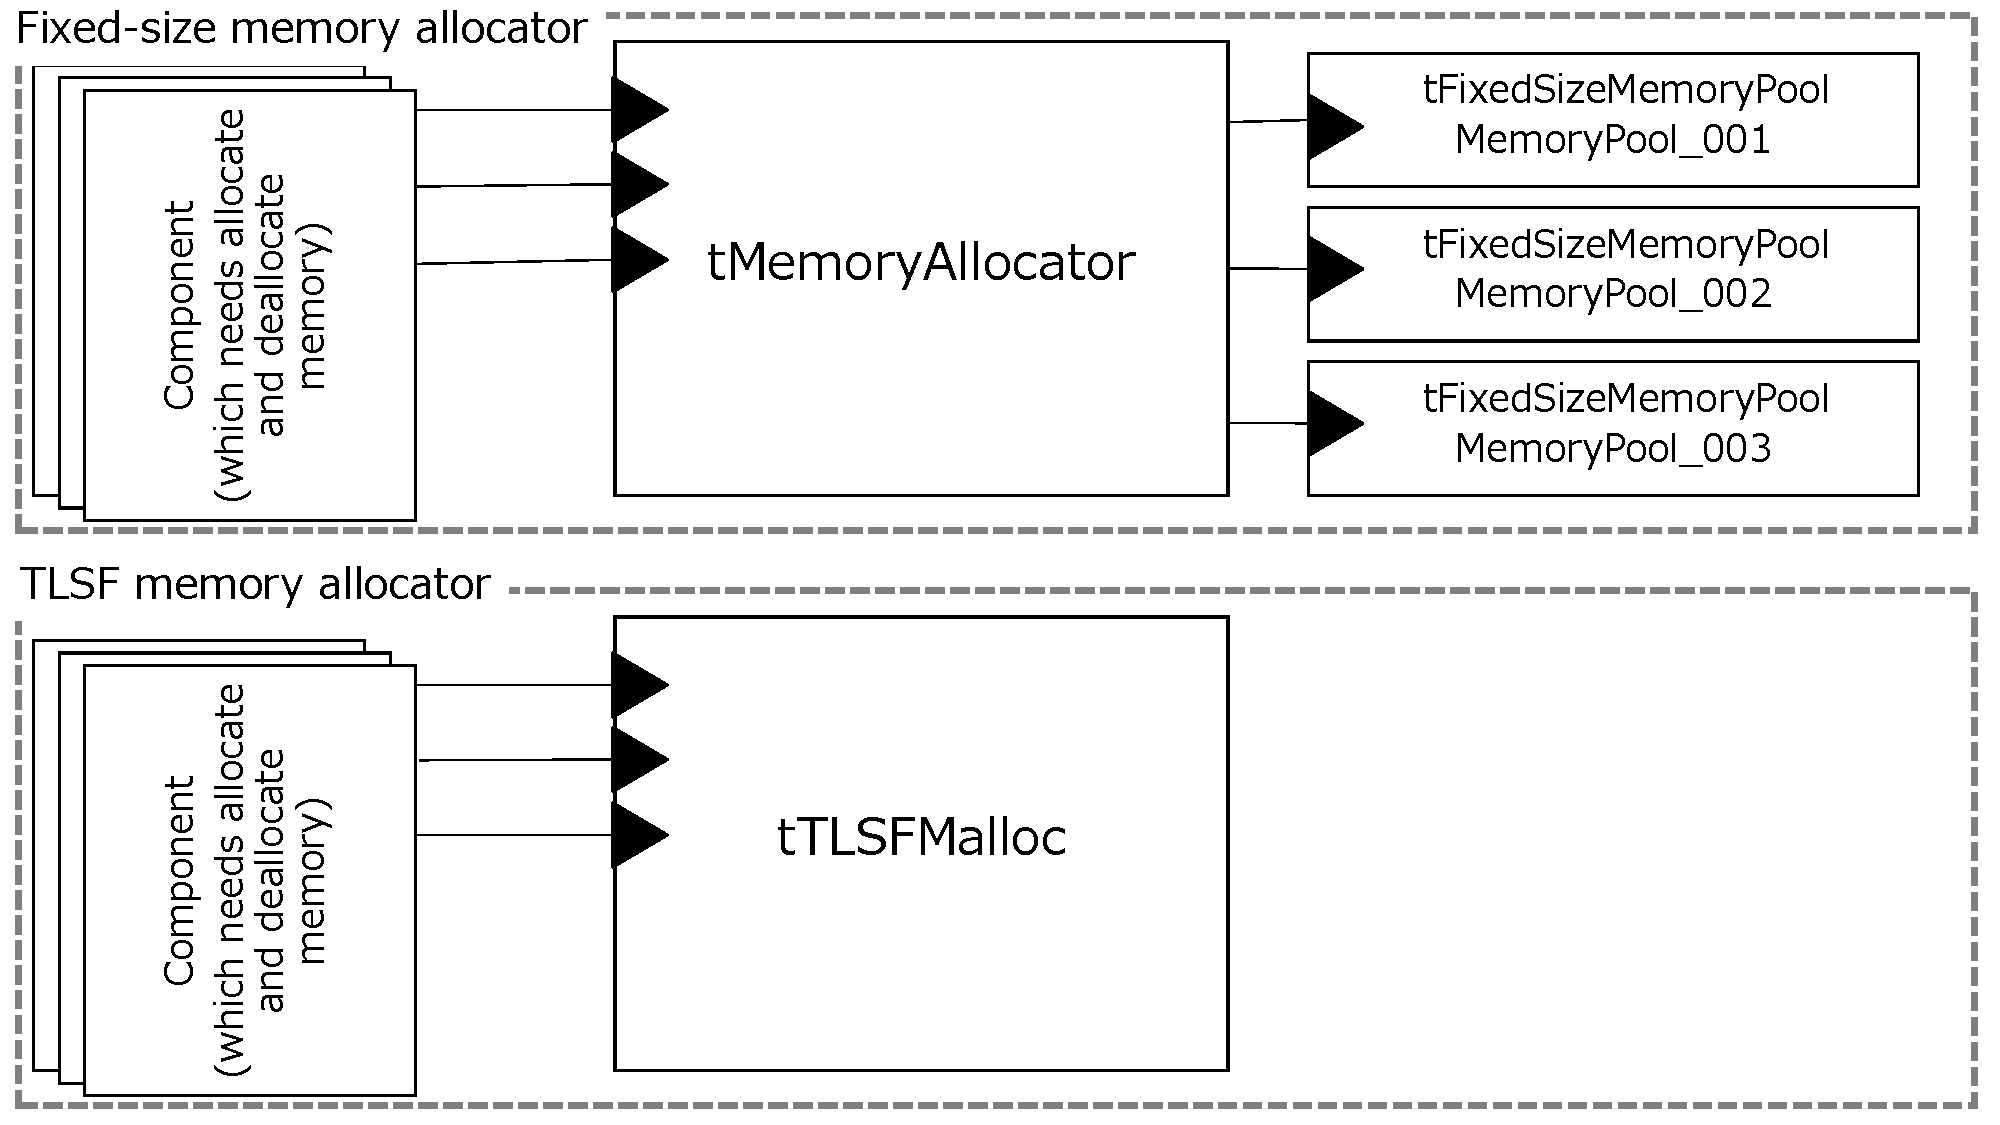
\includegraphics[width=8cm,clip]{figure/UseCase_TINET.pdf}
    \caption{固定長メモリアロケータとTLSFメモリアロケータ}
    \label{fig:UseCase_TINET}
\end{figure}
    

% \section{関連研究}
% \label{sec:RelatedWork}

\section{おわりに}
\label{sec:Conclusion}

本論文では,リアルタイムシステムに適した動的メモリアロケータであるTLSFメモリアロケータのコンポーネント化を提案した.
提案するコンポーネント化されたTLSFメモリアロケータは独自のヒープ領域を保持できるため,複数のスレッドから同時にメモリの確保や解放を行っても,メモリ競合が起こすことがない.
ヒープ領域のサイズはコンポーネントの内部変数として設定するため,サイズ変更も容易になる.

提案するTLSFメモリアロケータは,コンポーネント化によって再利用性も向上している.
利用したいシステムのメモリアロケータ部分をTLSFコンポーネントに入れ替えるだけで,利用可能となる.
さらに,コンポーネント図によってシステムを可視化でき,複雑で大規模なシステムを把握することに役立つ.

今後は,提案するTLSFコンポーネントの拡張として,統計情報を取得できるような機能を提供する.
メモリ確保の頻度や残りのヒープ領域サイズ等の情報を取得することで,メモリ制約の厳しい組込みシステムのソフトウェア開発の一助になると考えている.

%%%%%%%%%%%% Reference %%%%%%%%%%%%%%%%%%%%%%%%%%%%%%%%%%%%%%%%%%%%%%
\bibliographystyle{ipsj_v2/UTF8/ipsjunsrt-e}
\bibliography{ref}

% \begin{biography}
% \profile{m,E}{情報 太郎}{1970年生.1992年情報処理大学理学部情報科学科卒業.
% 1994年同大学大学院修士課程修了.同年情報処理学会入社.オンライン出版の研究
% に従事.電子情報通信学会,IEEE,ACM 各会員.}
% %
% \profile{n}{処理 花子}{1960年生.1982年情報処理大学理学部情報科学科卒業.
% 1984年同大学大学院修士課程修了.1987年同博士課程修了.理学博士.1987年情報処
% 理大学助手.1992年架空大学助教授.1997年同大教授.オンライン出版の研究
% に従事.2010年情報処理記念賞受賞.電子情報通信学会,IEEE,IEEE-CS,ACM
% 各会員.}
% %
% \profile{h,L}{学会 次郎}{1950年生.1974年架空大学大学院修士課程修了.
% 1987年同博士課程修了.工学博士.1977年架空大学助手.1992年情報処理大学助
% 教授.1987年同大教授.2000年から情報処理学会顧問.オンライン出版の研究
% に従事.2010年情報処理記念賞受賞.情報処理学会理事.電子情報通信学会,
% IEEE,IEEE-CS,ACM 各会員.}
% \end{biography}

\end{document}
